\documentclass[11pt]{article}
\usepackage[margin=1in]{geometry}
\usepackage{amsmath,amsthm,amssymb}
\usepackage{float}
\usepackage{hyperref}
\usepackage{booktabs}
\usepackage{placeins}
\usepackage{graphicx}

\title{Problem Diagnosis}
\author{José I. Velarde Morales}

\begin{document}
\maketitle
\section{Problem Description}
In our last meeting, I brought up the problem that the optimization method would set $a=b=0$ whenever both $a$ and $b$ were decision variables. This didn't make sense because it would seem that the objective could be improved upon by paying out sometimes. The program we were running was: 

\begin{align}
    \min_{a,b,\pi} &\quad t + \frac{1}{\epsilon}\sum_k p_k \gamma_k\\
    \text{s.t.   } I^k &\geq a\hat{l}(\theta^k) + b, \forall k\\
    0 &\leq I^k \leq y, \forall k\\
    E[I] &\leq \bar{\pi}y\\
    \gamma_k &\geq l^k + E[I] -I^k -t, \forall k\\
    \gamma_k &\geq 0, \forall k
\end{align}

I found that the problem was caused by constraint (2). The program was issuing payouts, (ie $I^k >0$ for some $k$), but it wasn't changing the values of $a$ and $b$. However, the resulting payouts ended up being piecewise linear with a slope of one (see Figure 1 for an example). The intercept varied based on the premium constraint. Changing constraint (2) to $I^k = a\hat{l}(\theta^k) + b$ did give non-zero values for $a,b$, but the payout function ends up being strictly linear, and seemed to perform worse than the baseline (see Figure 2 for an example). 

\begin{figure}[H]
    \centering
    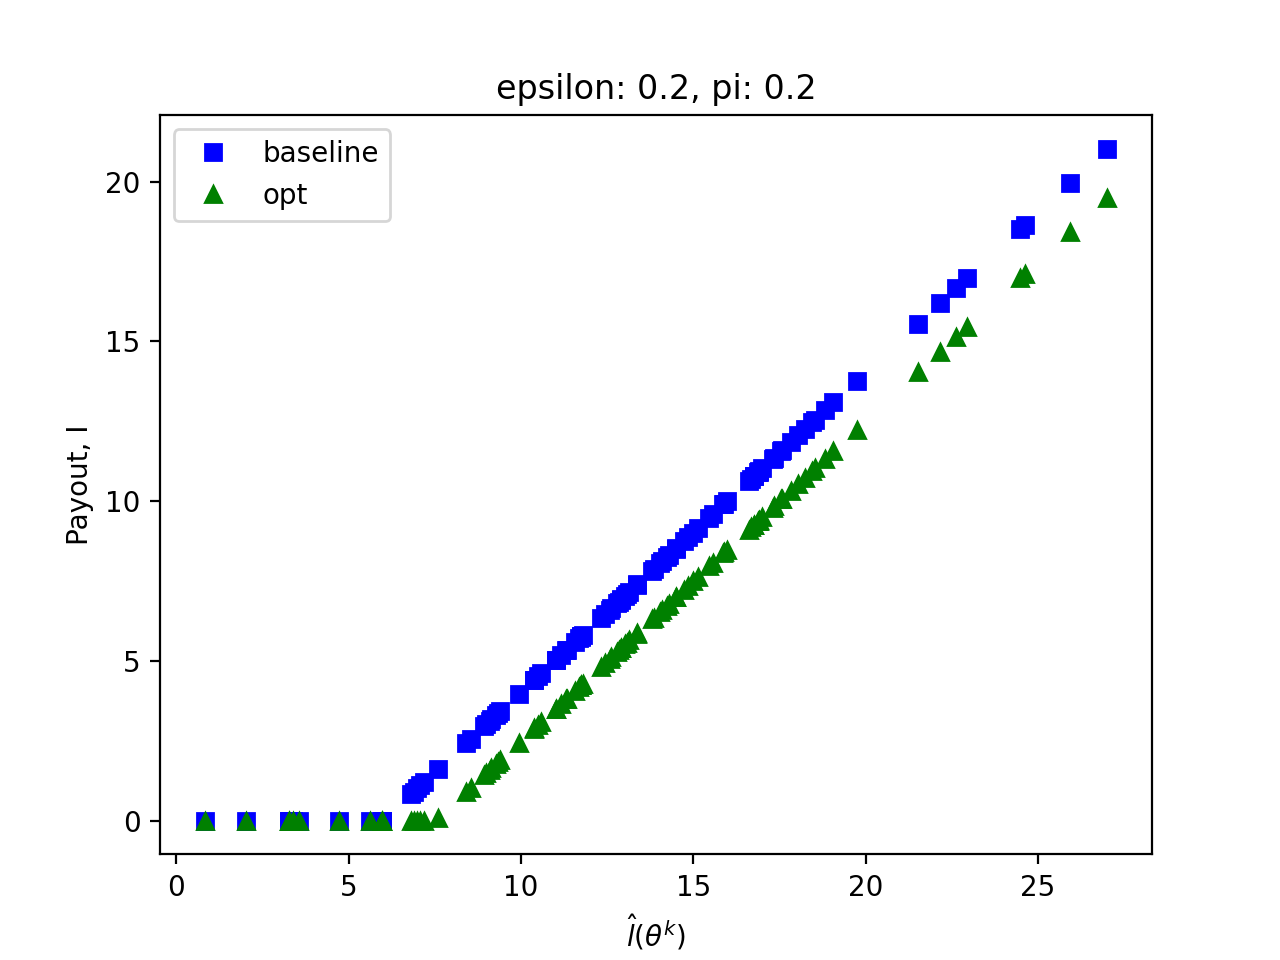
\includegraphics[width=0.65\textwidth]{eps_2_pi_2.png}
    \caption{Payout function when $\epsilon=0.2, \bar{\pi}=0.2$. This plots $I^k$ when we use the constraint $I^k \geq a\hat{l}(\theta^k) + b$}. 
\end{figure}

\begin{figure}[H]
    \centering
    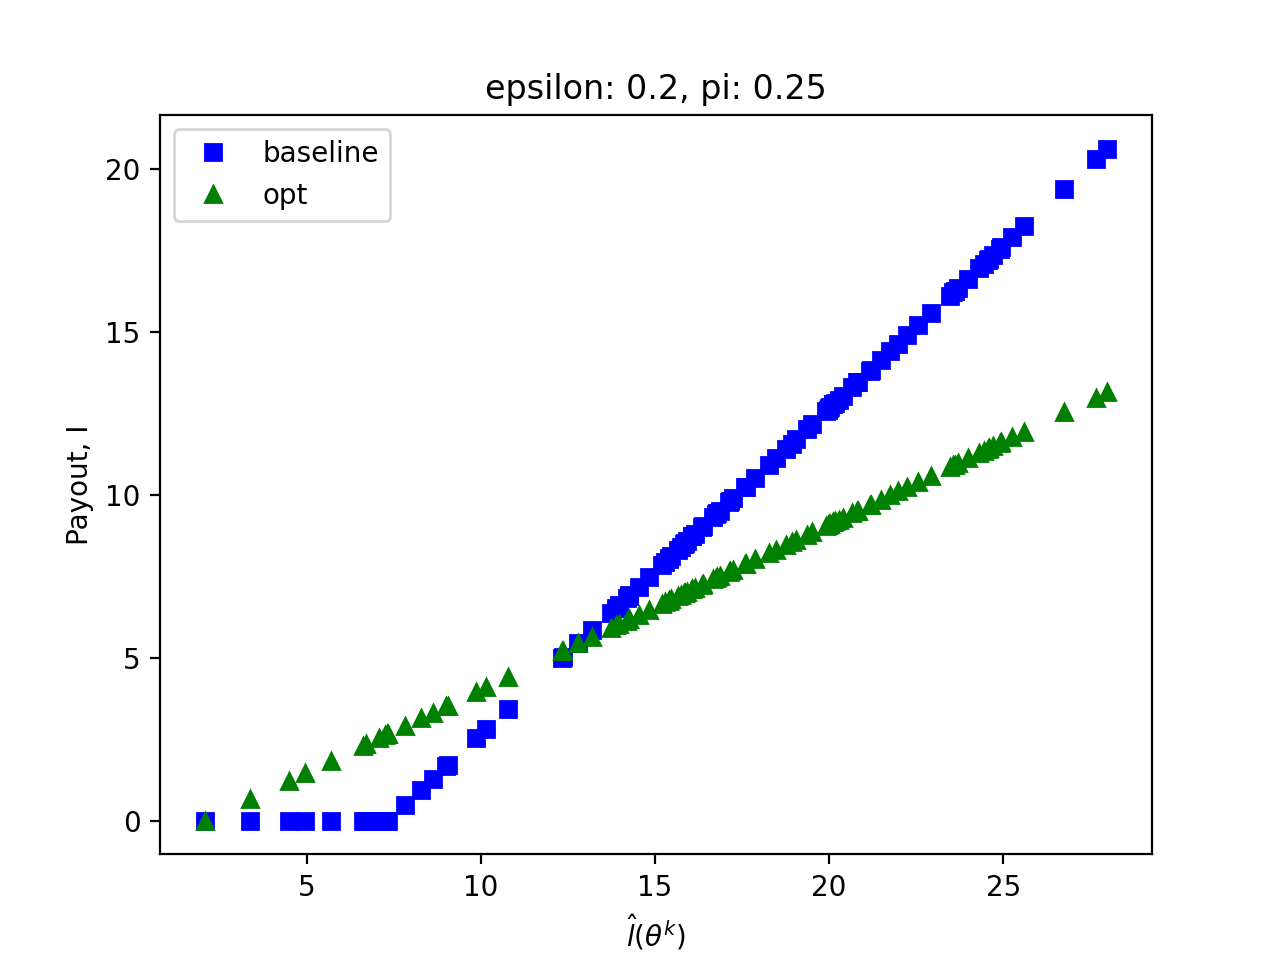
\includegraphics[width=0.65\textwidth]{linear_example.png}
    \caption{Payout function when $\epsilon=0.2, \bar{\pi}=0.25$. This plots $I^k$ when we use the constraint $I^k = a\hat{l}(\theta^k) + b$}. 
\end{figure}


\paragraph*{Idea for how to proceed}
\begin{itemize}
    \item One option would be to try to fit a piecewise linear function to the values of $I^k$ the program gives. We could set $b= \max \{\theta^k | I^k =0\}$, and we could calculate the slope of the function by running the following regression: $I^k = \beta \hat{l}(\theta^k)+\epsilon$, where we would only include observations where $I^k > 0$. However, I'm not sure if this is sketchy. 
\end{itemize}

\end{document}